\documentclass{article}
\usepackage[utf8]{inputenc}
\usepackage[margin=0.8in]{geometry} 
\usepackage{algorithm}
\usepackage{amsmath}
\usepackage{indentfirst}
\usepackage{amsmath}
\usepackage{graphicx}
\usepackage[noend]{algpseudocode}

\graphicspath{ {./images/} }

\title{\textbf{Tour Mate App}}
\author{
    Alexandre Abreu\\
    \texttt{up201800168@fe.up.pt}
    \and
    Eduardo Correia\\
    \texttt{up201806433@fe.up.pt}
    \and
    Juliane Marubayashi\\
    \texttt{up201800175@fe.up.pt}
}

\renewcommand{\today}{\ifcase \month \or January\or February\or March\or %
April\or May \or June\or July\or August\or September\or October\or November\or %
December\fi, \number \year}
\date{
    Faculdade de Engenharia da Universidade do Porto\\
    \today
}

\begin{document}

\maketitle

\section*{Keywords}

Tourism, Graph Theory, Network Graph

\section*{Abstraction}
    The goal of this project is to build the \textit{TourMateApp} application. \par
    This hypothetical application's purpose is to generate adaptable urban tourist routes, according to the personal preferences of its user.\par
    The methodology must use an implementation of graphs to get the values.

\section*{Introduction}
\subsection*{Problem Description}
    The problem discussed in this paper is how to evaluate the best tourist path to a client that is in a specific place and has limited time to spend, taking into account his preferences.\par
    We must take into account the time spend in commutations and the expected time of visits. \par
    For example reasons, we used the Porto city as a reference model to work on.

\section*{Model Formulation}
\subsection*{Edge Weight}
    The maximum speed and the distance to travel along an edge are used to calculate the cost of moving between two nodes, assuming there will be no interaction with other vehicles or people. \par

\subsection*{Input Data}
G = (V, E) - weighted directed graph:
\begin{itemize}
\item V - set of nodes representing points in the map:
    \begin{itemize}
    \item ID - unique, the id of the node in the Open Street Map.
    \end{itemize}

\item $E_i$ - edge representing a path between two nodes that is identified by the OSMid = i:
    \begin{itemize}
    \item $OSM id$ - the id of the edge in the Open Street Map.
    \item $S_i$ - The id of the source node.
    \item $T_i$ - The id of the target node.
    \item $L_i$ - Length of the road.
    \item $M_i$ - The maximum speed of the road.
    \item $O_i$ - True if the street is just one way, False otherwise.
    \end{itemize}
\end{itemize}

\subsection*{Input extraction from csv}
To initially obtain the map data from OSMnx \cite{OSMnx} we used a Python library that retrieves, models, analyzes, and visualizes street networks and other spatial data from OpenStreetMaps \cite{OpenStreetMaps}. \par
On that way, we can easily obtain a visual representation of streets and locations much like a graph - in which the crossings/POIs would be vertexes and the streets would be edges - and export it to a file our algorithm could parse. \par
Furthermore, the user would inform about its preferences, according to its trip purpose (recreational, work...), such as the list of POIs to visit, the maximum total time available to spend, the type of circuit (by foot, bicycle, car, public transportation...).

The input data includes \textit{.csv} files (obtained with OMSnx library \cite{OSMnx} and cleaned with Pandas \cite{Pandas}) stores information about the edges and nodes. \newline

\subsection*{Output Data}
    \subsubsection*{Output data available for the user}
    \begin{itemize}
        \item The path to pass by in order to achieve the points of interest as the path line shown on the map.
        \item Name of the streets and directions needed to be followed in respective order.
        \item The total time to be spent by the tourist, including visiting the POIs, and in the way to get to the places.
        \item The total distance to go.
    \end{itemize}

    \subsubsection*{Output data after loading files}
    After reading the \textit{.csv} file with edges and nodes information, a \textit{Dense Direct Graph} $G(V,E)$ will be built with $V$ vertexes and $E$ edges. In order to describe the output graph, consider $\lambda(i,j)$ as the direct cost between vertexes $i$ and $j$ and $w_{ij}$ as the weight between these two, with the following formal definition:

    \begin{equation}
      \lambda(i,j) =
        \begin{cases}
          \inf & \text{if i and j are not directly connected}\\
          w_{ij} & \text{if i and j are directly connected}\\
        \end{cases}
    \end{equation}

    \subsubsection*{Vertexes}
    \begin{itemize}
        \item $id$: vertex number identification.
        \item $Adj_i: $ adjacent list for a vertex i, $Adj_i \subseteq E$  , where $(j \in V \wedge j \neq i \wedge \lambda(i,j) < \inf) \rightarrow (j \in Adj_{i})$.
    \end{itemize}

    \subsubsection*{Edges}
    \begin{itemize}
        \item $S_{ref}$: source node reference
        \item $T_{ref}$: target node reference
        \item $w_{ij}$: calculated by $max\_velocity/road_{lenght}$
        \item name: name of the street
    \end{itemize}

\subsection*{Objective Function}

The optimal solution of the problem resides in minimizing the total time spent in commuting and the total traveled time and maximizing the number of points of interest visited. \par

\begin{itemize}
    \item $f = \sum_{t_{POI}}^{T} \Delta \lambda$, the total time spent in the POIs
    \item $g = \sum_{t_{travel}}^{T} \Delta \lambda$, the total time spent travelling
\end{itemize}
\and

\subsection*{Constraints}
\begin{itemize}
    \item $\lambda(i,j) > 0 \text{, } \forall (i,j) \in E$
    \item $ g > 0 \wedge f > 0$
    \item $T_{i} \neq NIL \wedge T_{ref} > 0 \text{, } \forall T_{ref} \in V$
    \item $S_{i} \neq NIL \wedge S_{ref} > 0 \text{, } \forall S_{ref} \in V$
    \item $L_{i} > 0$
    \item $M_i > 0$
\end{itemize}


\section*{Identification of Supported Cases}
    Considering the initial options given in the main menu of the application, the supported cases includes:
    \begin{itemize}
        \item Different types of locomotion: bus, on foot and car.
        \item The client can choose the points of interesting

    \end{itemize}
\section*{Solution Description}
\subsection*{Data Treatment}

\subsection*{Algorithms}
    The main algorithm to be used in the application is the \textit{Floyd Warshall} \cite{IntroductionToAlgorithms} \cite{FloydWarshal}. \par

    \begin{algorithm}[h]
    \caption{Floyd-Warshall}\label{euclid}
    \begin{algorithmic}[1]
    \Procedure{Shorthest Path}{G=(V, E)}
        \State $dist \gets N \times N \text{ matrix}$

        \For{\textbf{each} $\text{vertex } v \in dist$}
            \State $dist[i][i] \gets 0$
        \EndFor

        \For{\textbf{each} $\text{edge } w \in dist$}
            \State $dist[u][v] \gets weight(u, v)$
            \State $pred[u][v] \gets origin(w)$
        \EndFor

        \For{k \textbf{from} 1 \text{to} V}
            \For{i \textbf{from} 1 \text{to} V}
                \For{j \textbf{from} 1 \text{to} V}
                    \If{dist[i][j] $>$ dist[i][k] + dist[k][j]}
                        \State dist[i][j] = dist[i][k] + dist[k][j]
                        \State pred[i][j] = pred[k][j];
                    \EndIf
                \EndFor
            \EndFor
        \EndFor
    \EndProcedure
    \end{algorithmic}
    \end{algorithm}

    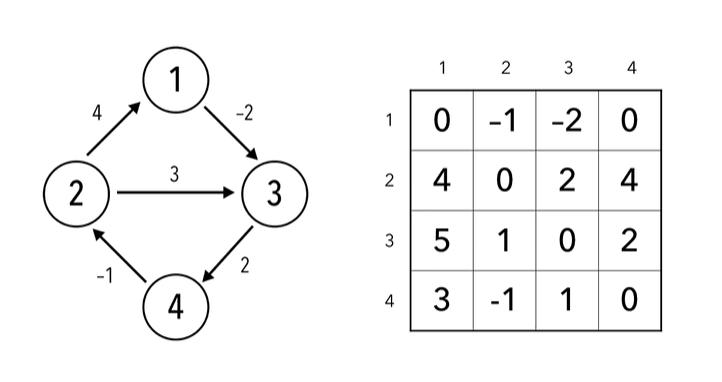
\includegraphics{algorithm-diagram}

    This algorithm considers the intermediate nodes to find and store all the shortest \b{distance} between nodes $i$ and $j$ with $k$ as intermediate vertex ($i \rightarrow k \rightarrow j$, which can simply described by the recursion formula:

    \begin{equation}
      d_{ij}^{(k)} =
        \begin{cases}
          w_{ij} & \text{if k = 0}\\
          min(d_{ij}^{k-1}, d_{ik}^{k-1} + d_{ki}^{k-1}) & \text{if } k\>= 1\\
        \end{cases}
    \end{equation}

    Besides the $O(|V^3|)$ complexity, this is a good approach for dense graphs like city networks.
    However, the \textit{Floyd Warshall} algorithm doesn't store the path between nodes. To do so, we can consider a new matrix called $\Pi$. \par
    For each $d_{ij}^{k}$ element in the matrix of shortest path $D^k$ the matrix $\Pi$ will contain the respective shortest path for the pair of nodes $i$ and $j$. \par
    Formally, each element of $\Pi$ can be described as it follows for $k>1$:

    \begin{equation}
      \pi_{ij}^{(k)} =
        \begin{cases}
          \pi_{ij}^{k-1} & \text{if } d_{ij}^{k-1} <= d_{ik}^{k-1} + d_{kj}^{k-1} \\
          \pi_{kj}^{k-1} & \text{if } d_{ij}^{k-1} > d_{ik}^{k-1} + d_{kj}^{k-1}\\
        \end{cases}
    \end{equation}

    For $k = 0$ the definition will be:

    \begin{equation}
      \pi_{ij}^{(0)} =
        \begin{cases}
          NIL & \text{if } w = \inf \vee \text{ i = j}\\
          i & \text{if } i \neq j \wedge w < \inf\\
        \end{cases}
    \end{equation}

    To complete the algorithm analysis, the spacial complexity for this algorithm should be $O(|v^2|)$, since it uses two auxiliary N $\times$ N matrixes. \newline
    In order to make the waiting time less significant, improvements to this algorithm will be considered.

\subsection*{Data Structures}
\subsubsection*{Nodes.csv}
        The \textit{nodes.csv} file is a simple table of one column with all the nodes in the graph identified by it's id.

\subsubsection*{Edges.csv}
\begin{itemize}
    \item $S_i$: Source, the id of the source node.
    \item $T_i$: Target, the id of the target node.
    \item $L_i$: Length of the road (in meters).
    \item $OSM id$: the id of the edge in the Open Street Map.
    \item $Name$: name of the street in which the node belongs.
    \item $O_i$: Oneway, if the street is just one way.
    \item $M_i$: Maxspeed, the maxspeed of the road (in kilometres per hour).
\end{itemize}

\section*{Conclusion}

The goal of this project was to develop a solution of the problem of route planning in a city sightseeing context. For that purpose we resort to shortest-path and optimization algorithms as well as dynamic programming.

\begin{thebibliography}{9}

\bibitem{OSMnx}
Boeing, Geoff, \textit{OSMNnx}, https://geoffboeing.com/publications/osmnx-complex-street-networks/

\bibitem{OpenStreetMaps}
\textit{Open Street Maps}, https://www.openstreetmap.org/

\bibitem{Pandas}
\textit{Pandas}, https://github.com/pandas-dev/pandas

\bibitem{IntroductionToAlgorithms}
Cormen, Thomas H., and Thomas H. Cormen. 2001. \textit{Introduction to algorithms}. Cambridge, Mass: MIT Press.

\bibitem{FloydWarshal}
Sambol, Michael, \textit{Floyd-Warshal Algorithm in 4 minutes}, https://www.youtube.com/watch?v=4OQeCuLYj-4

\end{thebibliography}

\end{document}

https://www.overleaf.com/project/5e7e00fdae8f9200012cd123